% Created 2018-06-21 Thu 12:30
\documentclass[8pt]{beamer}
\usepackage[sc,osf]{mathpazo}   % With old-style figures and real smallcaps.
\linespread{1.025}              % Palatino leads a little more leading
% Euler for math and numbers
\usepackage[euler-digits,small]{eulervm}
%\documentclass[10pt]{llncs}
%\usepackage{llncsdoc}
\usepackage{minted}
\usepackage[utf8]{inputenc}
\usepackage[T1]{fontenc}
\usepackage{fixltx2e}
\usepackage{graphicx}
\usepackage{longtable}
\usepackage{float}
\usepackage{wrapfig}
\usepackage{rotating}
\usepackage[normalem]{ulem}
\usepackage{amsmath}
\usepackage{textcomp}
\usepackage{marvosym}
\usepackage{wasysym}
\usepackage{amssymb}
\usepackage{hyperref}
\usepackage{polynom}
\renewcommand{\mod}[1]{\left( \texttt{mod}~#1 \right)}
\newcommand{\Z}{\mathbb Z}
\newcommand{\C}{\mathbb C}
\newcommand{\degree}{\texttt{degree}}
\tolerance=1000
\usetheme{Antibes}
\author{Siddharth Bhat}
\date{October 10th, 2019}
\institute{IIIT Theory group \\ Seminar Saturday}
\title{An introduction to the $p$-adics}
\hypersetup{
  pdfkeywords={},
  pdfsubject={},
  pdfcreator={Emacs 24.5.1 (Org mode 8.2.10)}}
\begin{document}

\maketitle

\begin{frame}[label=sec-1]{Why p-adics?}
Analogy between:
\begin{itemize}
\item $\mathbb Z$, \pause where $3, 5, 7, \dots$ are the ``primes''\pause
\item $\mathbb C[X]$, \pause where $(x - a)$ are the ``primes''
\end{itemize}
\end{frame}

\begin{frame}{What is evaluation?}

Remainder when dividing $p(x) = x^3 + x^2 + x + 1$ by $q(x) = x - 1$? \pause
\polylongdiv{X^3+X^2+X+1}{X-1}
\pause
$$(x^3+ x^2 + x + 1) = (x-1)(x^2 + 2x + 3) + 4$$
\pause
\begin{itemize}
\item $p(1) = 1^3 + 1^2 + 1 + 1 = 4$. Coincidence? \pause
\item Factoring out $q(x) = (x-1)$ \pause $ \simeq $ setting $q(x) = 0$ \pause : remove $q(x)$. \pause
\item setting $x - 1 = 0$, or setting $x = 1$ \pause
\item Substituting $x = 1$:  $p(1) = 1^3 + 1^2 + 1 + 1 = 4$ \pause
\end{itemize}

$$
\text{remainder of $p(x)$ on factoring $(x - a)$} \simeq \text{evaluation of $p(x_0)$ at $x_0 = a$}
$$
\end{frame}

\begin{frame}{What is evaluation in $\Z$?}

$$\text{remainder of $p(x)$ on factoring $(x - a)$} \simeq \text{evaluation of $p(x_0)$ at $x_0 = a$}$$
\pause
$$\text{evaluation of $p(x_0)$ at $x_0 = a$} \simeq \text{remainder of $p(x)$ on factoring $(x - a)$} $$
\pause
\begin{itemize}
\item $10(2)$ \pause $ = $ remainder of $10$ when factored by $2$; \pause $10 = 2\cdot5 + 0$\pause; $10(2) = 0$ \pause
\item $10(3)$ \pause $ = $ remainder of $10$ when factored by $3$; \pause $10 = 3\cdot3 + 1$ \pause; $10(3) = 1$ \pause
\item $10(5)$ \pause $ = $ remainder of $10$ when factored by $5$; \pause $10 = 5\cdot 2 + 0$ \pause; $10(5) = 0$ \pause
\item $10(7)$ \pause $ = $ remainder of $10$ when factored by $7$; \pause $10 = 7\cdot1 + 3$ \pause; $10(7) = 3$ \pause
\end{itemize}
\pause

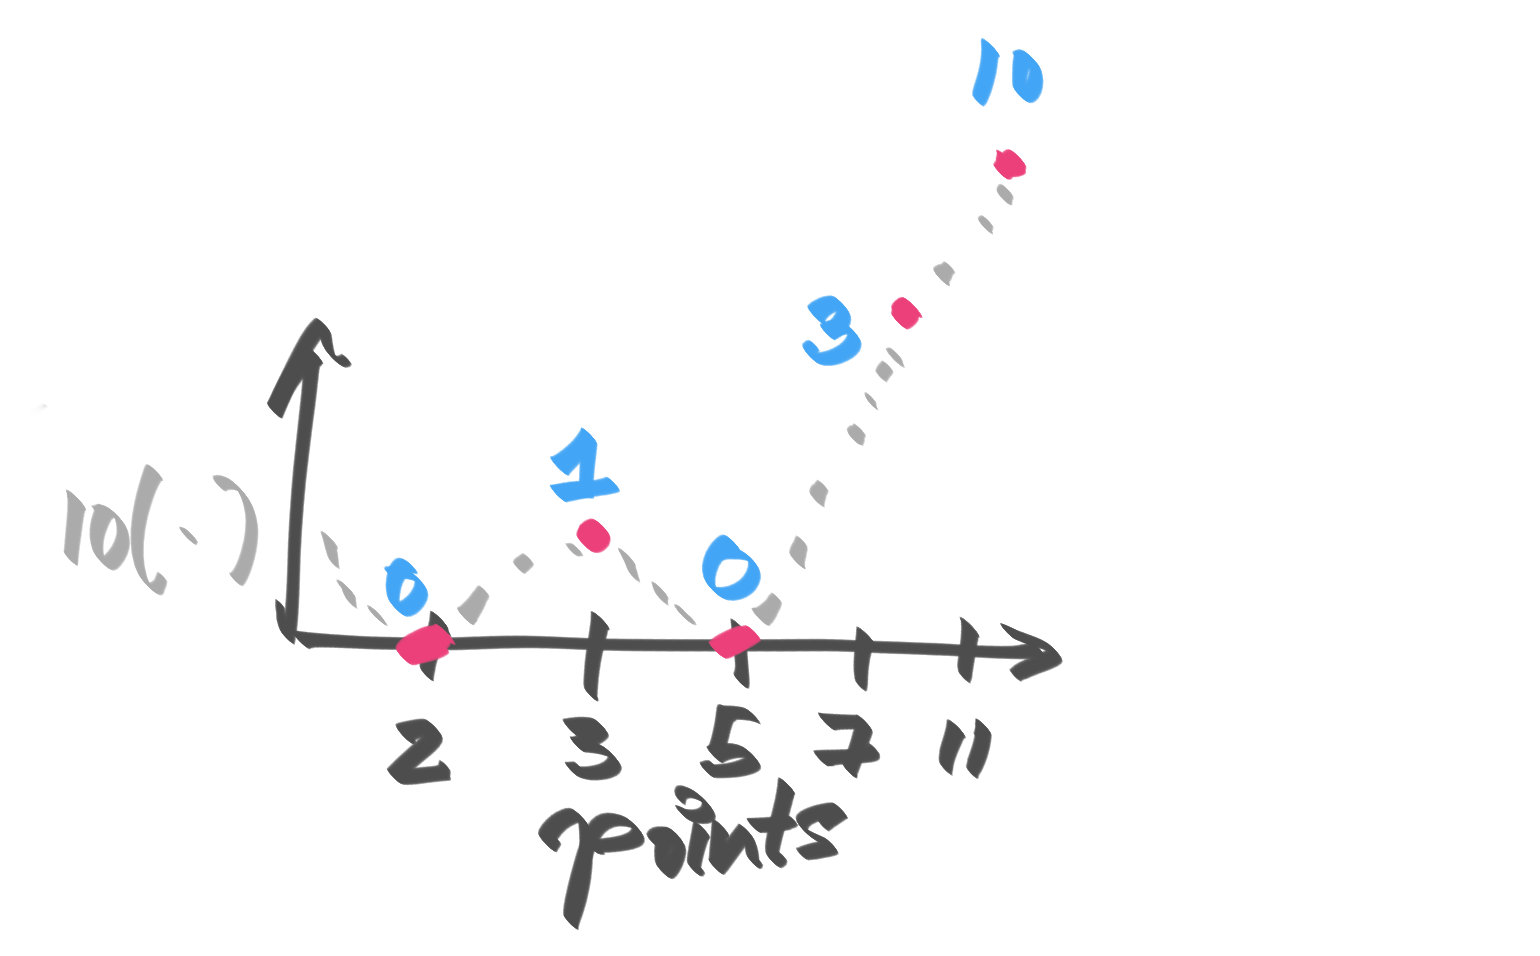
\includegraphics[width=3cm, height=3cm]{./10-as-a-fn.png}

\end{frame}

\begin{frame}{Why $n(p)$: only primes?}
\begin{itemize}
\item $10(5) = $ remainder of $10$ when factored by $5$; $10 = 5\cdot 2 + 0$ ; $10(5) = 0$
\item $10(7) = $ remainder of $10$ when factored by $7$; $10 = 7\cdot1 + 3$  ; $10(7) = 3$
\end{itemize}
\begin{itemize}
\item $p(x) = (x^2 - 15x + 50)$. \pause
\item $p(5) = $ \pause remainder of $p(x)$ when factored by $(x - 5)$; \pause 
\item $p(x) = (x-5)(x-10) + 0$; \pause $p(5) = 0$ \pause
\item $p(1) = $ \pause remainder of $p(x)$ when factored by $(x - 1)$; \pause 
\item $p(x) = (x-1)(x - 14) + 36$; \pause $p(1) = 36$ \pause
\end{itemize}

\pause

\begin{theorem}[Fundamental theorem of algebra] 
Every nonconstant polynomial $p(x) \in \C[X]$ can be written uniquely (upto reordering) as
a product of monic irreducibles of the form $(x - z_i)$ for $z_i \in C[X]$.
$$p(x) = \pm 1 \prod_i (x - z_i)$$
\end{theorem}

\pause

\begin{theorem}[Fundamental theorem of arithmetic] 
Every non-zero integer can be written uniquely (upto reordering) as a product of primes
$$n = \pm 1 \prod_i p_i$$
\end{theorem}

\end{frame}

\begin{frame}[fragile]{Cheap trick?}

\begin{itemize}
\item What are the complex numbers? \pause
\item $\mathbb R$ with $i$: $i^2 = -1$. \pause That is, $i^2 + 1 = 0$. \pause
\item Equivalently: $\mathbb R[X]$ \pause divided by $q(x) = x^2 + 1$. \pause
\item Left with only linear polynomials. \pause
\item All higher power polynomials $h(x)$  are $h(x) = p(x) \cdot q(x) + r(x)$ \pause $\degree(r) \leq 1$. \pause
\item Example: $7x^2 + 5 = 7(x^2 + 1) - 2$ \pause
\item Sum of linear polynomials: $(a + xb) + (c + xd) = (a + c) + x(b + d) $\pause
\item Product of linear polynomials: $(a + xb) \cdot (c + xd) = ac + x(ad + bc) + bdx^2$ \pause
\item dividing product by $q(x) = x^2 + 1$:
\end{itemize}

\polylongdiv{bd x^2 + (ad + bc) x + ac }{x^2+1} \pause

\begin{block}{This is what we expect: Complex multiplication}
$(a + bi) (c + di) = (ad + bc) i + (ac - bd)$
\end{block}
\end{frame}

\begin{frame}{Taylor series}

\begin{itemize}
\item Taylor series of $q(x) \in \C[X]$ at $x = x_0$: $q(x) = \sum_i a_i (x - x_0)^i$ \pause
\item Taylor series of $n \in \Z$ at $p$ prime: $n = \sum_i b_i p^i$. \pause
\end{itemize}
\begin{definition}
The $p$-adic expansion of a natural number $n$ is
the unique decomposition $n = \sum_i b_i p^i$ for $0 \leq b_i < p$.
\end{definition}

\begin{itemize}
\item Taylor series of $q(x) = x^3 - 7x^2 + 15x - 9$  \pause at $x = 3$: \pause $q(x) =  2(x - 3)^2 + (x - 3)^3$ \pause
\item $q(x) = (x-3)^2(2 + (x-3))$ \pause $ = (x-3)^2(x-1)$ \pause
\item $x^3 - 7x^2 + 15x - 9$ has a root at $3$ of order $2$ \pause

\item Taylor series/p-adic expansion of $72$ at $p = 3$: \pause $72 = 0 \cdot 3 + 2 \cdot 3^2 + 2 \cdot 3^3$ \pause
\item $72 = 3^2 * (2 + 2 \cdot 3) = 3^2 * 2^3$ \pause
\item $72$ has a root at $p=3$ of order $2$ \pause
\end{itemize}
\end{frame}

\begin{frame}{Extending to the negatives}

\begin{itemize}
\item Consider $-1$. \pause
\item Goal: write $-1 = a_0 3^0 + a_1 3^1 + a_2 3^2 + a_3 3^3 + \cdots$.
\item $-1 \equiv -1 + 3 - 3$. \pause
\item $-1 \equiv 2 - 3$ \pause
\item $-1 \equiv 2 - 3 + 9 - 9$ \pause
\item $-1 \equiv 2 + (9 - 3) - 9$ \pause
\item $-1 \equiv 2 + 6 - 9$ \pause
\item $-1 \equiv 2 + 6 - 9 + 27 - 27$ \pause
\item $-1 \equiv 2 + 6 + (27 - 9) - 125$ \pause
\item $-1 \equiv 2 + 6 + 100 - 125$ \pause
\item $-1 \equiv 2 \cdot 3^0 + 2 \cdot 3^1 + 2 \cdot 3^2 + \cdots$. \pause
\end{itemize}
\end{frame}

\begin{frame}[fragile]{Checking our math: $-1 + 1$}

\begin{itemize}
\item $-1 \equiv 2\cdot 3^0 + 2\cdot 3^1 + 2 \cdot 3^2 + 2 \cdot 3^3 + \cdots$. \pause
\item $-1 +1 = \mathbf{1 + 2\cdot 3^0} +   + 2\cdot 3^1 + 2 \cdot 3^2 + 2 \cdot 3^3 + \cdots$. \pause
\item $-1 +1 = \mathbf{1 \cdot 3^1 + 2\cdot 3^1} + 2 \cdot 3^2 + 2 \cdot 3^3 + \cdots$. \pause
\item $-1 +1 = \mathbf{1\cdot 3^2 + 2 \cdot 3^2} + 2 \cdot 3^3 + \cdots$. \pause
\item $-1 +1 = \mathbf{1\cdot 3^3 + 2 \cdot 3^3} + \cdots$. \pause
\item $-1 +1 = \cdots$ \pause
\item $-1 +1 = 0$.
\end{itemize}
\end{frame}
\begin{frame}[fragile]{Positional notation}

\begin{columns}% [T] % align columns
\begin{column}{.23\textwidth}
\begin{minted}{text}

...22222
...00001 + 
----------
...?????
----------
\end{minted}
\end{column}
%
\begin{column}{.23\textwidth}
\pause
\begin{minted}{text}
      1
...22222
...00001 + 
----------
       0
----------
\end{minted}
\end{column}
%
\begin{column}{.23\textwidth} 
\pause
\begin{minted}{text}
     1 
...22222
...00001 + 
----------
      00
----------
\end{minted}
\end{column}
%
\begin{column}{.23\textwidth} 
\pause
\begin{minted}{text}
      
...22222
...00001 + 
----------
...00000
----------
\end{minted}
\end{column}
\end{columns}
\pause

\begin{itemize}
\item What is $-1$ is $2$ - adically? \pause
\item $-1 = \dots 11111$. \pause
\item Same as $2$'s complement!
\end{itemize}
\end{frame}

\begin{frame}{Rationals}
\begin{itemize}
\item Evaluate $1/4$ in the $3$-adic system. \pause
\item $1/4$ \pause $ = 1/(1+3)$ \pause $ = 1 - 3 + 3^2 - 3^3 + 3^4 + \dots$\pause
\item What is $-3$? that's not allowed! \pause
\item $3^2 = 3 \cdot 3$ \pause
\item $1/4 = 1 - 3 + 3\cdot 3 - 3^3 + 3^4 + \cdots$ \pause
\item $1/4 = 1  + 2\cdot 3 - 3^3 + 3^4 + \cdots$ \pause
\item $1/4 = 1  + 2\cdot 3 - 3^3 + 3\cdot 3^3 + \cdots$ \pause
\item $1/4 = 1  + 2\cdot 3 + 2\cdot 3^3 + \cdots$ \pause
\item Similar cleverness produces $1/p$ for any rational. \pause
\end{itemize}
\end{frame}


\begin{frame}{Irrationals?}
\end{frame}


\begin{frame}{Convergence}
\end{frame}

\begin{frame}{A lemma of Hensel}
\end{frame}

\begin{frame}[fragile]{Why only primes? Geometry}
\begin{itemize}
\item Dividing $p(x)$ by $(x-a_0)$ $\simeq$ evaluating  $p(x)$ at $x = a_0$ \pause
\item Dividing $z \in \mathbb Z$ by $a_0 \in \mathbb Z$ $\simeq$ evaluating $z$ at $a_0$? \pause
\item $f(x)$: continuous, emph{non-zero} at $x = a_0$. \pause
\item $f(x)$: \emph{invertible} around $x = a_0$. \pause
\item consider $6$. \pause
\item nonzero at $a_0 = 4$: $6 \simeq 2~\mod{4}$\pause
\item \emph{not invertible} in $(\mathbb{Z}/4\mathbb{Z})^\times$ \pause
\item $(\mathbb{Z}/n\mathbb{Z})^\times$:group iff $n$ prime
\end{itemize}

\end{frame}
\end{document}
